\documentclass[17pt]{extarticle}
\usepackage{greg}

\title{Towards Differential Geometry in Homotopy Type Theory}
\author{Greg Langmead}

\begin{document}
\maketitle
\begin{abstract}
This thesis will show how to formalize parts of differential geometry in homotopy type theory.\cite{freed2013chernweil} \cite{kobayashinomizu} \cite{hamilton2017} \cite{scorpan_wild_2005} \cite{baez1994gauge} \cite{atiyah1983yang}
\end{abstract}
\tableofcontents
\section{Introduction}
This thesis is very much in the spirit of Freed and Hopkins \cite{freed2013chernweil}, where the authors adopt the point of view of a classicial differential geometer and teach us how much we may gain by generalizing the standard constructions towards sheaves, towards groupoids, and towards simplicial sets. Homotopy Type Theory offers a formalism for working with these advanced objects, as do $\infty$-toposes. A community of folks have been evangelizing this higher-dimensional point of view for many years, explaining how we might use it to work with geometry and physics. I have managed to devote some time to following up on their suggestions.
\section{Manifolds to $\infty$-topos: SDG and beyond}
This section will explain how to fully and faithfully embed the category of smooth manifolds and smooth maps into a topos of $\infty$-sheaves of algebras.

\section{Groups, actions, and bundles}
\emph{Types $X$ over $BG$ are group actions.} We have the pointed connected type $BG$ with $\pt : BG$. Above $\pt$ we have $X(\pt)$, on which $G$ acts by transport: if $p : \pt=\pt$ then $tr(p): X(\pt) \to X(\pt)$, and this is a group action.

\emph{The dependent sum $(\alpha:BG)\times X(z)$ deserves to be called $X//G$.} I go back to my textbook and see that identities in any dependent sum, say between $(g, x)$ and $(h, y)$ are given by a pair: an equality $p:g=h$ in the base, and an equality in the fiber over $h$, $q:y=tr(p, x)$. In the group context such an equality means $x$ and $y$ are in the same orbit of the $G$-action, and so we have recorded the orbits with equalities, a groupoidification of the action.

\emph{The dependent product $(\alpha:BG)\to X(z)$ deserves to be called the space of fixed points of the action.} 

\subsection{Multiple delooping shenanigans}
Second delooping of a higher group is abelian: Lemma 2.1.6 in the HoTT book \cite{hottbook}.

\subsection{Principal bundles in HoTT}
Many of the benefits of using HoTT and $\infty$-toposes derive from the idea of \emph{universes}. A universe is a type inside of which are contained other types, a nesting that lets us talk more intuitively about classifying spaces. 

Consider the classical story of Grassmanians, which classify vector bundles. The Grassmanian $G(k,n)$ is the set of $k$-dimensional subspaces of $\rr^n$. There is a natural topology on this set which gives it the structure of a compact smooth manifold. It is the base space of a vector bundle $E(k,n)\to G(k,n)$, whose fiber over a point is the vector space at that point: $E(k,n) = \{(p, v): G(k,n)\times\rr^n | v\in p\}$. This construction was very circular and confusing to me as a classical mathematician, and the type theory formulation is not only a vast generalization, but a \emph{clarification}. The magic that's being perpetrated in the Grassmanian construction is that the base space $G$ has as its points entire vector spaces, but collapsed to a single point conceptually, and then the honest vector space as a set is installed over that point to form $E$. The base point in $G$ is the vector space considered as a single set: $G$ is a set of sets. This is already worthy of the name ``universe,'' and we should note that standard set theory permits such nesting.

Taking the union $\cup_{n=1}^{\infty}E(k,n)\to G(k,n)$ over all dimensions of ambient $\rr^n$s gives a bundle $E(k)\to G(k)$ whose spaces are infinite dimensional, with fiber having dimension $k$. Why do we have to pass to infinite dimensions? Only then can we formulate a clean theorem:
\begin{mythm}
	If $M$ is a paracompact topological manifold, then the map from homotopy classes of maps $[M, G(k)]$ to equivalence classes of $k$-dimensional vector bundles over $M$, $\mathrm{Vect}(M, k)$ given by pulling back $E(k)$, i.e. $[f]\mapsto f^*(E(k))$, is a bijection.
\end{mythm}
What if we imagined performing the construction $[M, G(k)]$ literally? In spirit it might be related to the project of embedding an abstract manifold $M$ in some $\rr^n$, which can always be done and for which there are strong bounds on the required dimension compared to the dimension of $M$ and various topological properties of $M$. In the case of classifying a bundle over $M$ we would be mapping $M$ into the less topologically trivial space of planes. There would be a lot going on if we were to really try this! For a fixed manifold we only need a finite-dimensional $G(k,n)$ to establish the bijection, but there are three factors that increase the bound on dimension as we consider every manifold and bundle. First there is obviously the dimension of the manifold, which can be arbitrarily large. Second, the manifold may have nontrivial topology which requires a very high dimensional space to make room for the necessary topological squirming. And third, a given vector bundle may itself be twisty over the topology of $M$ and require more dimensional room to capture it. Passing to the union of all the Grassmanians allows us to make the blanket statement.

But even classically that's not how we use the theorem. Its use is usually theoretical. We can use it to reduce questions about vector bundles to questions about the universal bundle, so long as the construction we're attempting is preserved by the pullback. That is just what happens in type theory with universes. They help understand structures over types by studing maps from types into a universe. \gc{strengthen this parallel if possible}

The theory of vector bundles leads to the more general theory of principal bundles, and there's a lossless passage back and forth in the case of vector bundles provided by considering frame bundles...\gc{discuss frame bundles}


\section{Finding the manifolds inside HoTT}
\section{Effective epimorphisms}
Classically, effective means information is not lost. If two points get glued together we retain that there were two points by having a self-arrow. One of points turned into an arrow. There is conservation of mass (if points and arrows have equal mass).

In HoTT, functions are automatically mass-conserving, so a function can only fail to be an effective epi if it fails to be an epi. The only way to fail to be an epi is to miss a point. In HoTT, we define surjections as points with merely inhabited fibers, so these don't miss any points. Putting this all together, in HoTT all surjections are effective epis. They will interpret to effective epis in the categorical semantics.

\section{Back to manifolds: local triviality and freeness for free}
\begin{mythm}
	Let $(\alpha:BG): P(\alpha)$ be a type family over the delooping of a higher group $G$. If we interpret this type family in $\formalsmoothset$ such that $P$ and $G$ are 0-types and honest manifolds, then we obtain a classical smooth principal bundle $G\to P \to P/G$. In particular, $G$ acts freely on $P$ and the bundle is locally trivial.
\end{mythm}

\subsection{Honest manifolds}
If we decide to interpret HoTT in \formalsmoothset, then how can we locate, or define, the types that will interpret onto the actual smooth manifolds? Remember that we enlarged the category tremendously along two dimensions: first we moved to sheaves, then we added higher structure.

So for one thing, smooth manifolds lack higher structure and so will be among the 0-types. It remains therefore to find the non-exotic, or manifoldy, 0-types.

Let's recall the original definition of a smooth manifold. A modern and category-theory-aware textbook for differential geometry is \cite{kolar_natural_1993}, so this might be a good place to start. I'll paraphrase their definition a little:

\begin{mydef}
A topological manifold is a separable Hausdorff space $M$ which is locally homeomorphic to $\rr^n$. So for any $x\in M$ there is an open neighborhood $U$ of $x$ and a map $u:U\to \rr^n$ that is a homeomorphism onto its image which is an open subset of $\rr^n.$ Such maps are called coordinate charts.A covering family $\{U_\alpha, u_\alpha\}$ of coordinate charts is called an atlas. An atlas is called a smooth atlas if the compositions that can be formed between $\rr^n$ are smooth (that is, $C^\infty$). Finally, a smooth manifold is a topological manifold with a smooth atlas.
\end{mydef}
``The compositions that can be formed'' means the usual business of composing charts and the inverse of charts whenever the charts overlap on $M$, forming homeomorphisms between open sets in $\rr^n$.

I remember reading definitions like this and glossing over the words ``separable'', ``Hausdorff'', and the fine print about the charts being homeomorphic to an open subset of $\rr^n$. I could tell that $n$ was being chosen to match the dimension of the manifold, and secretly I was probably also assuming $M$ is connected so that $n$ could be constant rather than just locally constant. But this intellectual debt is about to be paid, because these are precisely the restrictions that we need to define internally in HoTT to find the manifolds, and so we will need to understand them a bit better.

Let's look next at the definition of smooth manifold that's in use in the mathlib library of Lean. Here, manifolds are defined to be instances of \texttt{charted\_space}\cite{charted_space} which is the same as an atlas: every point is contained in an open neighborhood that is the domain of a \texttt{local\_homeomorph}, i.e. a homeomorphism to an open subset of a fixed vector space over a fixed field.

\subsection{Local triviality is absorbed}

\subsection{Freeness is absorbed}

\subsection{Structures requiring groupoids are absorbed, e.g. connections}

\section{You will see if we gained anything}

\section{Notes from 6/23/2021 meeting}
Effective epis. An effective epi is intuitively a map that preserves all the information. Every point goes somewhere, every morphism goes somewhere, every 2-morphism etc. This is apparently what a homotopy colimit is too, and so that's why we say the map is the colimit of its simplicial diagram. When a groupoid acts it can be non-effective if it discards some of the equivalences and maps points to the same point without also preserving the arrow as a self-arrow. Conservation of mass. In HoTT, all the higher structure is always preserved, and so the only reason a map can fail to be an effective epi is if it fails to be surjective, i.e. fails to hit some point, i.e. the fiber over some point is empty. Since a surjection is defined as a map with all nonempty fibers, all surjectives are effective epi in HoTT.

Submersions. In Diff, the category of smooth manifolds, pullbacks do not exist, but a pullback ``along a submersion'' does. Surjective submersions are regular epis. Ehresmann's theorem: a proper submersion is a locally trivial fibration. (Proper: sends compact subsets to compact subsets.) Surjective submersions form a ``singleton Grothendieck pretopology'' on Diff. These generate a G-topology. Coverages are a weaker notion that also generate a G-topology. A G-topology is a coverage satisfying: being stable under pullback, stable under composition, and that isomorphisms form a cover. The term ``singleton'' in this context simply means that the covering families each contain a single map.

Surjective submersions are precisely the local-section-admitting maps: https://mathoverflow.net/questions/40309/in-diff-are-the-surjective-submersions-precisely-the-local-section-admitting-ma

Aside: good open covers pull back just to open covers, and so are not G-topology.

Claim: effective epis in HoTT will interpret to surjective submersions in the case where the codomain is a smooth manifold. Note that a surjective submersion is precisly a map with local sections, as surjectivity of the derivative can be extended locally to a map in the reverse direction.

Local trivializations: One definition of locally trivial map we are proposing is: $E\to X$ is locally trivial there exists an effective epi $Y\to X$ such that the pullback of the bundle is trivial, i.e. isomorphic to a product. 
% https://q.uiver.app/?q=WzAsNCxbMSwwLCJFIl0sWzEsMSwiWCJdLFswLDEsIlkiXSxbMCwwLCJZXFx0aW1lcyBGIl0sWzAsMSwicCJdLFszLDIsIlxcbWF0aHJte3ByfV8xIiwyXSxbMiwxLCJmIiwyXSxbMywwLCJcXGNvbmciXSxbMywxLCIiLDEseyJzdHlsZSI6eyJuYW1lIjoiY29ybmVyIn19XV0=
\[\begin{tikzcd}
	{Y\times F} & E \\
	Y & X
	\arrow["p", from=1-2, to=2-2]
	\arrow["{\mathrm{pr}_1}"', from=1-1, to=2-1]
	\arrow["f"', from=2-1, to=2-2]
	\arrow["\cong", from=1-1, to=1-2]
	\arrow["\lrcorner"{anchor=center, pos=0.125}, draw=none, from=1-1, to=2-2]
\end{tikzcd}\]

Given a trivializing effective epi (LEE) then we want to eventually interpret this in 0-types that behave like smooth manifolds and show the link with classical local triviality. We will use
\begin{mylemma} If $X$ is a manifold object in the topos of SmoothSet, and $p:X'\to X$ is an effective epi, then the map has local sections (via the inverse/implicit function theorem):
% https://q.uiver.app/?q=WzAsMyxbMSwwLCJYJyJdLFsxLDEsIlgiXSxbMCwxLCJcXGNvcHJvZCBVX2kiXSxbMCwxLCJcXGZvcmFsbCBcXG1hdGhybXtlZmZcXCBlcGl9Il0sWzIsMSwiXFxtYXRocm17b3BlblxcIGNvdmVyfSIsMl0sWzIsMCwiXFxleGlzdHMgXFxzaWdtYSJdXQ==
\[\begin{tikzcd}
	& {X'} \\
	{\coprod U_i} & X:\mathsf{Diff}
	\arrow["{\forall \mathrm{eff\ epi}}", from=1-2, to=2-2]
	\arrow["{\mathrm{open\ cover}}"', from=2-1, to=2-2]
	\arrow["{\exists \sigma}", from=2-1, to=1-2]
\end{tikzcd}\]
\end{mylemma}
\begin{proof}
    We need to step down from sheaves to manifolds. Why do effective epis in the topos context specialize to surjective submersions on a representable?
\end{proof}

Candidates for the definition of ``open cover''.

1. A subset of effective epis that are a) stable under composition (a cover of a cover is a cover, which is apparently called a $\Sigma$-condition) because
% https://q.uiver.app/?q=WzAsNCxbMCwxLCJVIl0sWzEsMSwiWCJdLFswLDAsIlYiXSxbMSwwLCJcXHN1bV9VIFZfVSJdLFswLDEsIlxcbWF0aHJte2NvdmVyfSIsMl0sWzIsMCwiXFxtYXRocm17Y292ZXJ9IiwyXSxbMiwzLCJcXHNpbWVxIl0sWzMsMSwiXFxtYXRocm17XFx1bmRlcmxpbmV7XFx1bmRlcmxpbmV7Y292ZXJ9fX0iXV0=
\[\begin{tikzcd}
	V & {\sum_U V_U} \\
	U & X
	\arrow["{\mathrm{cover}}"', from=2-1, to=2-2]
	\arrow["{\mathrm{cover}}"', from=1-1, to=2-1]
	\arrow["\simeq", from=1-1, to=1-2]
	\arrow["{\mathrm{\underline{\underline{cover}}}}", from=1-2, to=2-2]
\end{tikzcd}\]
and b) stable under base change (which we will get for free in HoTT?).

2. A subset of opens inside the object classifier $\Omega$. Also a definition of an open map. We might call the special collection of opens ``blocks''. We would interpret them onto the $\rr^n$s. We call a type $X$ \emph{geometric} with respect to these opens if there is an \emph{open} map $\coprod_i U_i \to X$. These are the spaces that can be built by gluing together the blocks. In the interpretation it will sit in a chain of inclusions $$\mathrm{Manifolds}\subset \mathrm{Geometric} \subset \mathrm{Diffeological} \subset \mathrm{Sh}(\rr^n)$$

One of the non-manifolds that are geometric would be two copies of $\rr$ glued everywhere but at the origin, so a real line with two origins. This is geometric. But what is not geometric is the union of the $x$ and $y$ axes in $\rr^2$. Here the maps from $\rr$ are not open maps.

Submersions: These are smooth maps that locally look like projections from $\rr^{n+k}\to \rr^n$. A Morse function is not a submersion. A bundle map is a submersion. The map $x^3-y^2:\rr^2\to \rr$ is not a submersion because the fibers change topology due to singularities.

Discussion of the manifold objects inside the Cahiers topos: https://mathoverflow.net/questions/79514/what-are-the-smooth-manifolds-in-the-topos-of-sheaves-on-a-smooth-manifold

Principal bundles in HoTT, a review. Mike's blog post about classifying spaces: https://golem.ph.utexas.edu/category/2015/01/the_univalent_perspective_on_c.html. A dependent type $p:E\to B$ is given by a classifying map $E:B\to \mathrm{Type}$, and a principal bundle is one where $E$ factors through $BG$, so $E:B\to BG$. One way to define $BG$ is by $$\sum_{E:\mathrm{Type}^G}||E\simeq_{\mathrm{Type}^G} G||_{-1}$$, where $\mathrm{Type}^G$ is the universe of types equipped with a $G$-action. The action of $G$ on itself is via translation, i.e. left or right multiplication. I've been saying to myself that ``$BG$ is everything equal to $G$'' but this is more precise.

We have a surjection followed by a mono
% https://q.uiver.app/?q=WzAsNSxbMCwwLCIxIl0sWzEsMCwiQkciXSxbMiwwLCJcXG1hdGhybXtUeXBlfV5HIl0sWzMsMCwiXFxtYXRocm17VHlwZX0iXSxbMSwxLCJcXHN1bV97RTpcXG1hdGhybXtUeXBlfV5HfXx8RVxcc2ltZXFfe1xcbWF0aHJte1R5cGV9Xkd9IEd8fF97LTF9Il0sWzAsMSwiIiwxLHsic3R5bGUiOnsiaGVhZCI6eyJuYW1lIjoiZXBpIn19fV0sWzEsMiwiIiwxLHsic3R5bGUiOnsidGFpbCI6eyJuYW1lIjoibW9ubyJ9fX1dLFsyLDNdLFsxLDQsIiIsMSx7ImxldmVsIjoyLCJzdHlsZSI6eyJoZWFkIjp7Im5hbWUiOiJub25lIn19fV1d
\[\begin{tikzcd}
	1 & BG & {\mathrm{Type}^G} & {\mathrm{Type}} \\
	& {\sum_{E:\mathrm{Type}^G}||E\simeq_{\mathrm{Type}^G} G||_{-1}}
	\arrow[two heads, from=1-1, to=1-2]
	\arrow[tail, from=1-2, to=1-3]
	\arrow[from=1-3, to=1-4]
	\arrow[Rightarrow, no head, from=1-2, to=2-2]
\end{tikzcd}\]

Trivializing principal bundles. What are the fibers of $p$? 
% https://q.uiver.app/?q=WzAsNyxbMywxLCJCR1xcc3Vic2V0XFxtYXRocm17VHlwZX0iXSxbMywwLCJCIl0sWzQsMCwiMSJdLFsyLDEsIjEiXSxbMiwwLCJcXHN1bV9iXFxtYXRocm17SWR9KEYsRV9iKSJdLFsxLDAsIlAiXSxbMCwwLCJcXHN1bV9iXFxtYXRocm17SWR9KEcsRV9iKSJdLFs0LDNdLFszLDAsIkYiXSxbNCwxXSxbMSwwXSxbNCwwLCIiLDEseyJzdHlsZSI6eyJuYW1lIjoiY29ybmVyIn19XSxbMSwyXSxbNiw1LCIiLDEseyJsZXZlbCI6Miwic3R5bGUiOnsiaGVhZCI6eyJuYW1lIjoibm9uZSJ9fX1dLFs1LDQsIiIsMSx7ImxldmVsIjoyLCJzdHlsZSI6eyJoZWFkIjp7Im5hbWUiOiJub25lIn19fV0sWzQsMV0sWzEsNCwiIiwyLHsib2Zmc2V0IjoyLCJjdXJ2ZSI6Miwic3R5bGUiOnsiYm9keSI6eyJuYW1lIjoiZGFzaGVkIn19fV1d
\[\begin{tikzcd}
	{\sum_b\mathrm{Id}(G,E_b)} & P & {\sum_b\mathrm{Id}(F,E_b)} & B & 1 \\
	&& 1 & {BG\subset\mathrm{Type}}
	\arrow[from=1-3, to=2-3]
	\arrow["F", from=2-3, to=2-4]
	\arrow[from=1-3, to=1-4]
	\arrow[from=1-4, to=2-4]
	\arrow["\lrcorner"{anchor=center, pos=0.125}, draw=none, from=1-3, to=2-4]
	\arrow[from=1-4, to=1-5]
	\arrow[Rightarrow, no head, from=1-1, to=1-2]
	\arrow[Rightarrow, no head, from=1-2, to=1-3]
	\arrow[from=1-3, to=1-4]
	\arrow[shift right=2, curve={height=12pt}, dashed, from=1-4, to=1-3]
\end{tikzcd}\]
where the dotted arrow is a putative section, i.e. a trivialization of the bundle.

Adopt the point of view: are the fibers of the bundle all equivalent? What type is the type of the fibers? If we know the typical fiber is $F$, then we can look at the total space of identifications between $F$ and the fiber. This is a dependent type over the base $B$. A section of this is a global choice of such an identification. I was surprised to learn that this is the same as a section of the bundle, a trivialization! But of course that tracks with the classical story: the fibers are only identifiable with $G$ once you choose a basepoint. To do that globally is exactly a section. So this is just recapitulating that idea, plus the fact that in HoTT sections are continuous.

Consider that $\sum_b\mathrm{Id}(G,E_b)$ is the type of all points $b:B$ in the base and identifications between $G$ and the fiber $E_b$. Identifications of the fiber with $G$, in the case where $G$ is the correct group, i.e. this type is inhabited, is exactly a copy of $E_b$ because the identification is the same as a choice of basepoint.

\section{Notes on Readings}
\subsection{Buchholtz, van Doorn, Rijke}
Background on connectedness from HoTT book 7.5: A type $A$ is $n$-connected if the unique function $A\to 1$ is $n$-connected (for all $b : 1$ we have $||\mathrm{fib}_f(b)||_n$ is contractible), i.e. if $||A||_n$ is contractible. If $A$ is -1-connected we say it is \emph{merely inhabited}. If it is 0-connected we say it is \emph{connected}, and if it is 1-connected we say it is \emph{simply connected}.

(Section 2) The type of pointed types is $\mathrm{Type}_\mathrm{pt}$. The homotopy groups of a pointed type are $\pi_k(A) = ||{\Omega_k(A)}||_0$ i.e. the zero-truncation (so, a set, a standard group) of the loop space.

(Section 3) The 1-loop map establishes an isomorphism between higher groups and pointed, connected types. Why connected? What is connected? Answer: connectedness is the truncation of contractibility: $\sum_{a:A}\prod_{x:A}||x=a||_{-1}$.

Being $n$-truncated means you have no nontrivial identities at level $n$ or above. $-2$-truncated means you are contractible. Being $n$-connected means you have no nontrivial identities below $n$, and so means your $n$-truncation $||A||_n$ is contractible. This is a generalization of the term ``simply connected''.

If $A$ is a pointed type (with designated point pt), its loop space is a higher group: $\Omega A := (\pt =_A \pt)$. There is something special happening with this. We are fully leveraging the infrastructure of the identity type, which obeys group laws up to coherences, in an infinite tower. We are designating this infrastructure to \emph{be} a group. So this is synthetic, using the identity types.

If $G$ is a group, then we write $BG$ for ``the'' type satisfying $G=\Omega BG$. We call $BG$ the delooping of $G$. The identification of $G$ and $BG$ connects groups to groupoids.

(Section 4) Given a type $A$ and $a : A$, we have $\Aut\ a := (a = a)$. Importantly, $\BAut\ a$ is the connected component of $a$, expressed as $\im(a : 1 \to A) = (x : A) \times ||a = x||_{-1}$. This product notation is Agda style for a dependent sum.

For example, consider $S_n$, the permutation group of $\Fin\ n$, which is a specific set with $n$ elements. Then $BS_n$ is the type of all $n$-element sets. This was rather mind-blowing to me at first. We started by installing the group as the automorphisms of just a single point, but along the way we obtained every equivalent object as well.

A group homomorphism is a pointed map $f: G \to H$ of groups and a pointed map $Bf: BG \to BH$ of the delooping, such that $\Omega Bf \sim f$.

There's a terse comment that if $h, k : G \to H$ are homorphisms between set-level groups, then they are conjugate (which I'm taking to mean that $hg = x(kg)x^{-1}$ for some $x\in H$) if the pointed maps $Bh, Bk: BG \to BH$ are freely homotopic, i.e. equal as unpointed maps $BG \to BH$. What I'm struggling with is that surely $Bh$ and $Bk$ must be pointed because $h$ and $k$ are maps between the same groups. Here is a picture from stackoverflow \gc{https://math.stackexchange.com/questions/2458349/base-point-homotopy-vs-free-homotopy-example} where two elements of the fundamental group are conjugate (by the green loop) and freely homotopic (where you are allowed to move the base point around the hole I guess?) but not homotopic.
\begin{figure}[H]
  \centering
  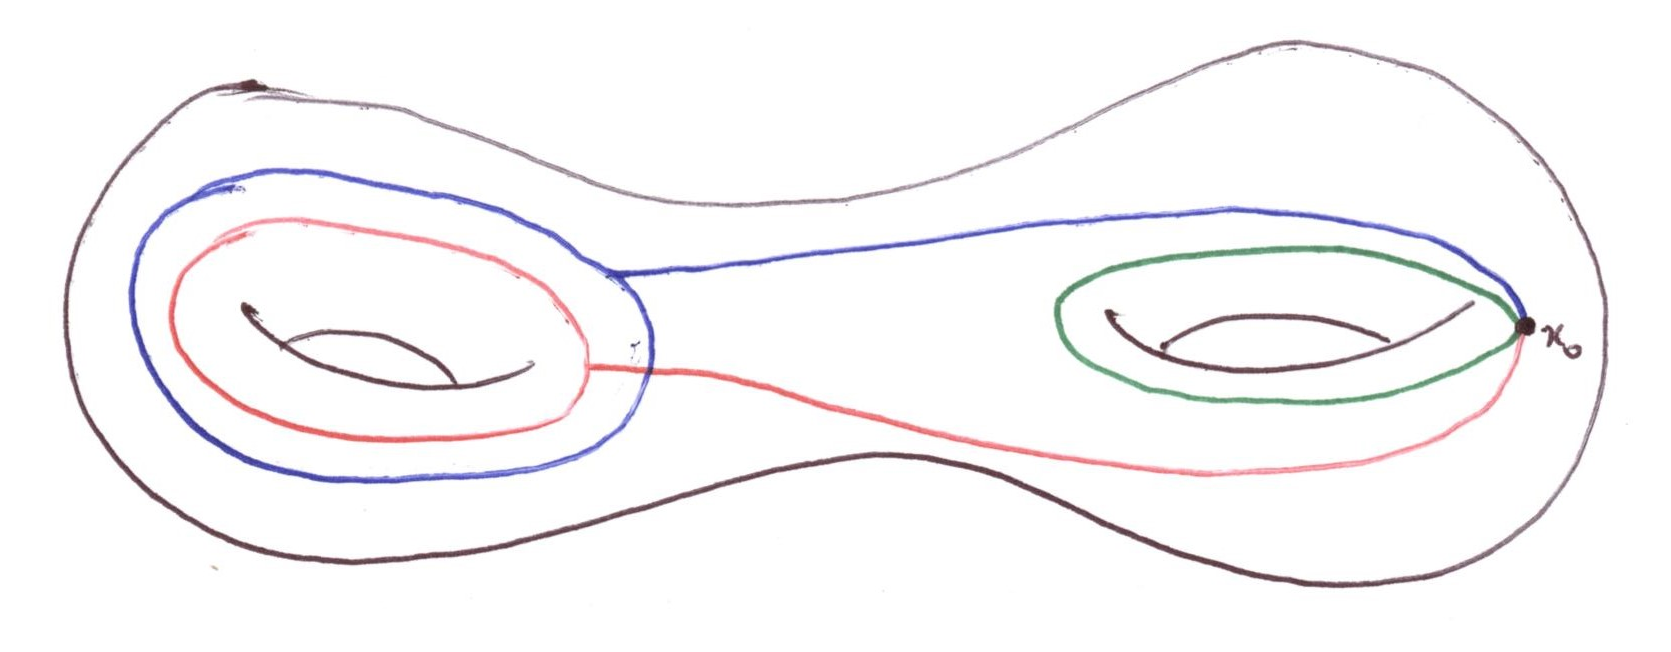
\includegraphics[scale=0.2]{conjugating_loops.png}
\end{figure}

If we have a family of pointed types over a pointed type, i.e. $X:\Type_{\pt}$ and $Y : X \to_{\pt} \Type_{\pt}$, then the type of \emph{pointed sections} is a section $s$ such that $s\ \pt = \pt$, i.e. we only specify this extra data at $\pt : X$. One canonical such section is the constant section $x \mapsto \pt : Y(x)$ and so this is itself a pointed type with the constant section as base point.

There are some lemmas about the levels of connectivity that hold for a space of pointed sections, given data about the connectivity of the base and fibers.

The action of a group $G$ on an object $a : A$ is a map $X: BG \to A$ with $X(pt) = a$. ``Clearly'' this is the same as a homomorphism $G \to \Aut_A a$. (Because a homomorphism is defined as a deloopable map and we just defined the action in terms of the delooping.)

A ``$G$-type'' is a type in the context of $BG$, i.e. a map $X : BG \to \Type$. A map of $G$-types is a function $\alpha : (z : BG) \to X(z) \to Y(z)$. This is a map for each point of $BG$. So we are calling $X$ the $G$-type, not the type $X(pt)$.

\subsection{Egbert on fixed points}
A higher group $G$ is defined to be a pointed connected type $BG$. The underlying type of the higher group $G$ is then just the loop space of $BG$. This loop space is what $G$ really is, and its group structure comes from it being the loop space of $BG$. A $G$-type should then be a type equipped with a $G$-action. We just define it as a fibration over $BG$, so that the $G$-action comes canonically from the lifting property. So, if $X : BG \to Type$, then we have

\begin{enumerate}
\item a type $X(*)$ at the base point
\item a G-action $X(*) \to X(*)$ for every loop of $BG$
\end{enumerate}

If $X$ would be a $G$-set, then the type of fixed points would be

$$\sum (x : X(*)), \prod (p : * = *), tr(p,x) = x$$

where tr is transport/lift. With a bit of abstract nonsense it follows that this is the type

$$\prod (y : BG), X(y).$$

However, if $X$ is not a $G$-set but a $G$-type, then that first type of fixed points isn't quite right, because it misses the higher coherences. It turns out that the Pi-type is the right thing :)

\subsection{Egbert on quotients by group actions}
So why do we define $X/G := \sum (y : BG), X(y)$? Quotients should have a quotient map: Here the quotient map is just the inclusion of the fiber $X(*)$. The quotient map is surjective: This follows from the fact that $BG$ is connected. The quotient map should be effective: in other words, in $X/G$ we should have

$$q(x)=q(y) \simeq \sum (g:G), gx=y$$

This identity type is a $\Sigma$-type. That's already the first hint that the quotient should be a $\Sigma$-type. And indeed a quick calculation will reveal that effectiveness indeed holds.

\bibliography{connections}
\end{document}